\subsection{SageMath: Uvod}

\paragraph{Kaj je SageMath (SageMath)?}

\begin{itemize}
\item SageMath (na kratko Sage) je brezplačen odprtokodni programski sistem za matematiko.
\item Lahko si ga predstavljate kot Phyton na matematičnih steroidih.
\item Poslanstvo sistema SageMath je ustvariti učinkovito brezplačno odprtokodno alternativo sistemom Magma, Maple, Mathematica in Matlab.
\end{itemize}

\begin{framed}
\textbf{Glej tudi}\\
SageMath se pogosto uporablja in na spletu je na voljo veliko gradiva. Navajam nekaj najuporabnejših virov.

\begin{itemize}
\item SageMath Documentation: \href{https://doc.sagemath.org/}{https://doc.sagemath.org/}
\item SageMath Reference Manual: \href{https://doc.sagemath.org/html/en/reference/index.html}{https://doc.sagemath.org/html/en/reference/index.html}
\item A tour of SageMath: \href{https://doc.sagemath.org/html/en/a\_tour\_of\_sage/}{https://doc.sagemath.org/html/en/a\_tour\_of\_sage/}
\item Introductory SageMath tutorial: \href{https://doc.sagemath.org/html/en/prep/Intro-Tutorial.html}{https://doc.sagemath.org/html/en/prep/Intro-Tutorial.html}
\item SageMath tutorial: \href{https://doc.sagemath.org/html/en/tutorial/index.html}{https://doc.sagemath.org/html/en/tutorial/index.html}
\item SageMath thematic tutorial: \href{https://doc.sagemath.org/html/en/thematic\_tutorials/index.html}{https://doc.sagemath.org/html/en/thematic\_tutorials/index.html}
\item SageMath repository of interacts (interaktivni programčki): \href{https://wiki.sagemath.org/interact}{https://wiki.sagemath.org/interact}
\item SageMath quickref cards (reference za pomoč): \href{https://wiki.sagemath.org/quickref}{https://wiki.sagemath.org/quickref}
\end{itemize}
\end{framed}

\paragraph{Kako uporabljamo SageMath?}

SageMath lahko uporabljate na več načinov, vsak od njih ponuja različno raven nadzora in različne funkcije. Glavni načini uporabe so:

\begin{itemize}
\item \textbf{SageCell} \href{https://sagecell.sagemath.org/}{https://sagecell.sagemath.org/} Zelo uporabno za enostavne in hitre naloge.
\item \textbf{Lokalna namestitev}. Ni priporočljivo za začetnike. Če nimate izkušenj z nameščanjem programske opreme, je to lahko nekoliko zapleteno. Poleg tega skoraj nikoli ni potrebna. Edini dober razlog za lokalno namestitev programa SageMath je, da nimate dostopa do interneta.
\item \textbf{Interaktivni programčki}. Podobno kot apleti GeoGebre. Za uporabo interaktivnih programčkov ni treba imeti predznanja. Za njihovo ustvarjanje pa potrebujete napredno poznavanje programa SageMath, ki presega vsebine tega predmeta.
\item \textbf{\href{http://CoCalc.com}{CoCalc.com}} \url{https://cocalc.com/}. S preprostimi besedami, CoCal je za SageMath, kar je Overleaf za LaTeX.
\end{itemize}

\paragraph{SageMath na CoCalcu}

Obstajajo različne načine za uporabo SageMath, najpogosteje so:

\begin{itemize}
\item Na ukazni vrstici (terminalu). Ta način je primeren za napredne uporabnike in ni priporočljiv za začetnike. V tem primeru, SageMath deluje podobno kot običajen programski jezik, ukaze napišemo v terminal in dobimo rezultate. Ukazna vrstica običajno izgleda kot Figure~\ref{fig-terminal}.
\end{itemize}

\begin{figure}[!htbp]
\centering
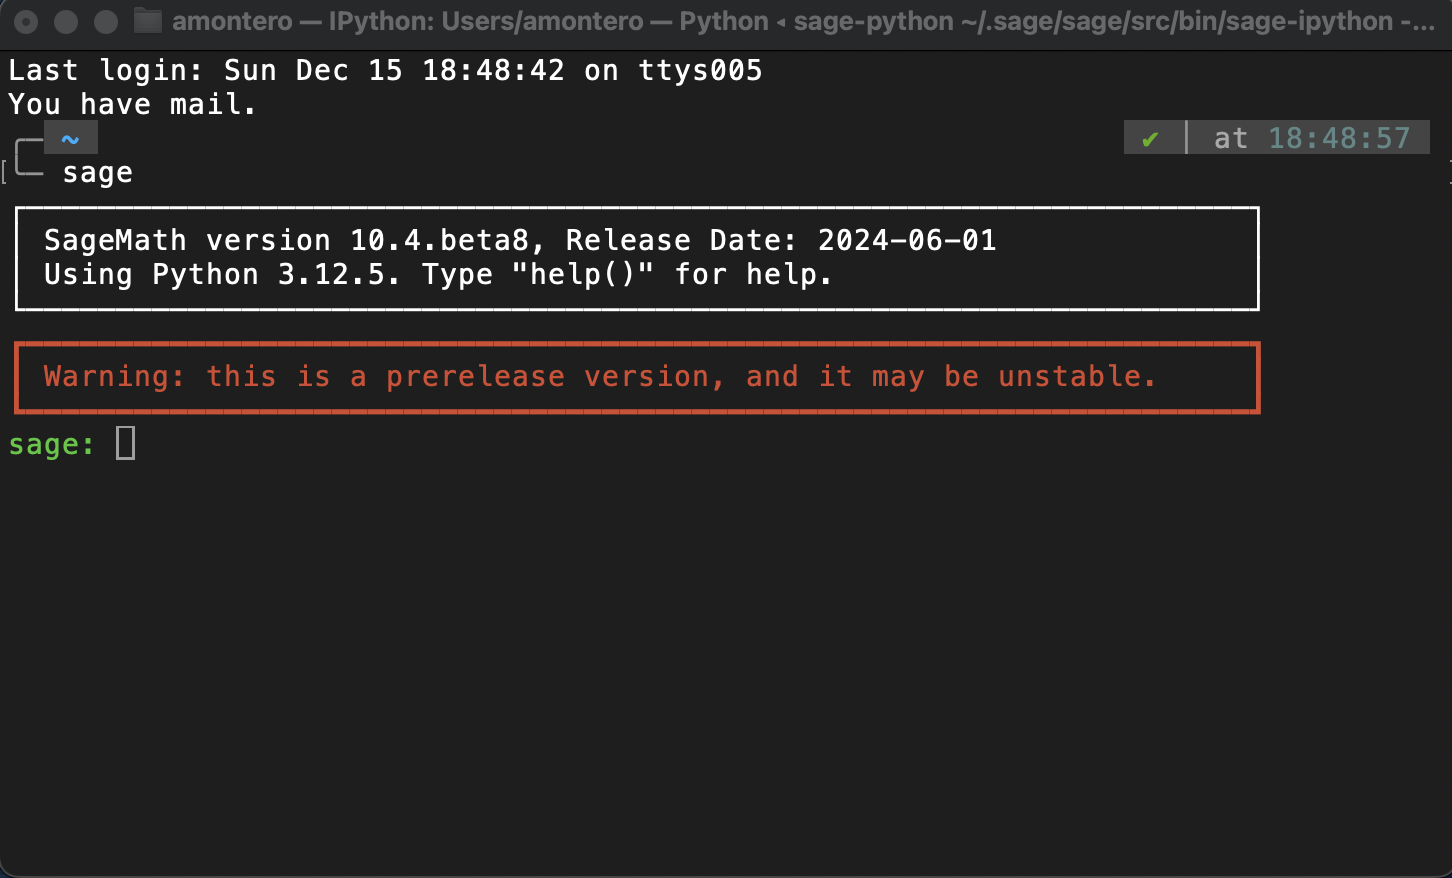
\includegraphics[width=0.5\linewidth]{files/terminal-e0334a7d9dbbd6f7e95e80a76bc04315.png}
\caption[]{Ukazna vrstica SageMath}
\label{fig-terminal}
\end{figure}

\begin{itemize}
\item Scripting: Kodo napišemo v besedilno datoteko in jo nato zaženete v ukazni vrstici. Ta način je prav tako primeren za napredne uporabnike in ni priporočljiv za začetnike, saj zahteva poznavanje osnov programiranja.
\item \textbf{Interaktivno v zvezku (Jupyter Notebook)}. Ta način je najbolj primeren za začetnike in je tisti, ki ga bomo uporabljali v tem predmetu. SageMath lahko uporabljamo v zvezkih Jupyter, ki omogočajo kombiniranje besedila, matematičnih izrazov in kode v enem dokumentu. Zvezki so zelo uporabni za učenje, raziskovanje in dokumentiranje matematičnih izračunov. V tem predmetu bomo uporabljali CoCalc, spletno platformo, ki omogoča uporabo SageMath v zvezkih Jupyter brez potrebe po lokalni namestitvi.
\end{itemize}

V beležnici Jupyter imamo dve vrsti celic: \textit{Code} (koda) in \textit{Text} (besedilo) (glej Figure~\ref{fig-celice}).

\begin{figure}[!htbp]
\centering
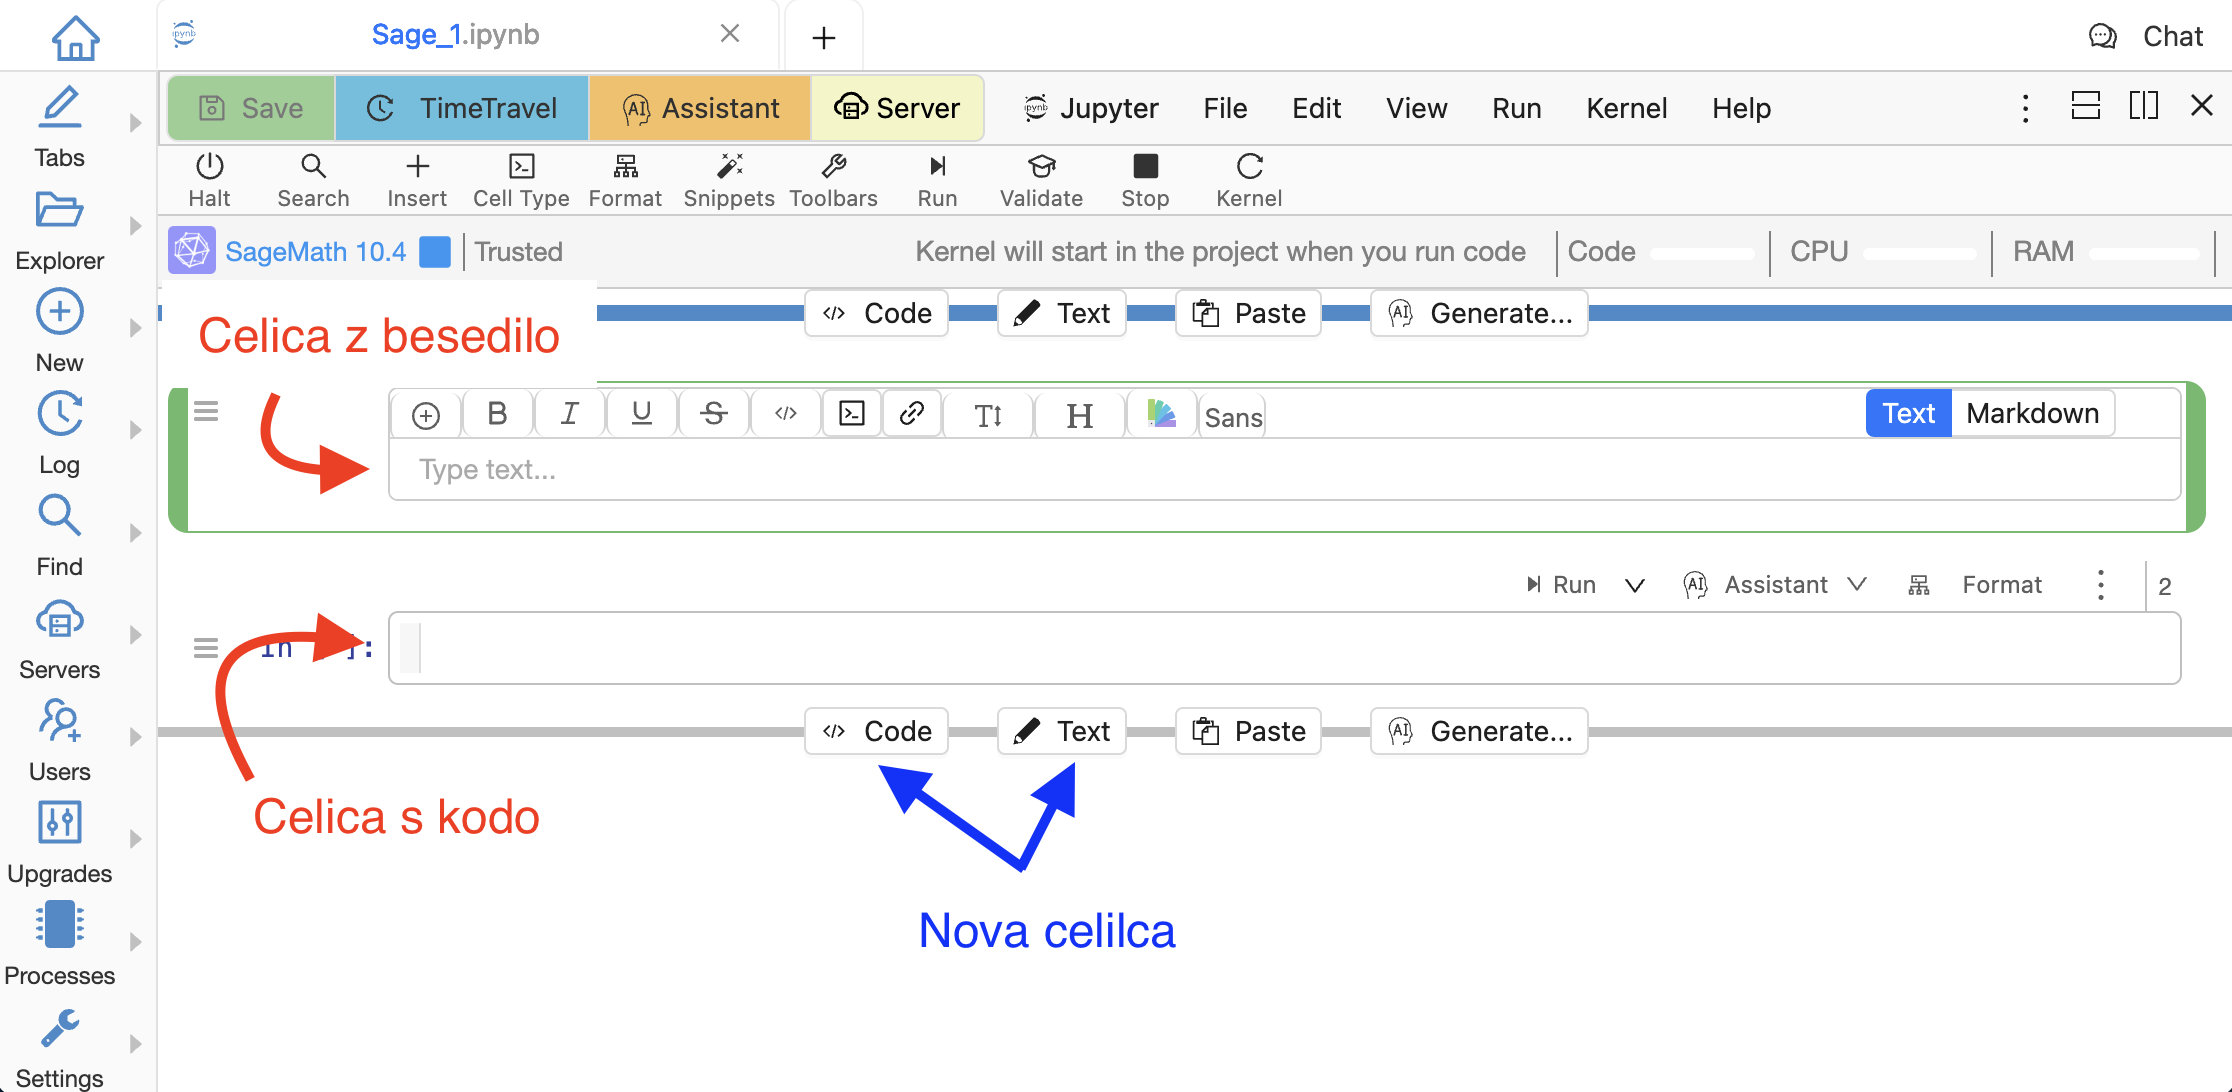
\includegraphics[width=0.5\linewidth]{files/jupyter4-93d3d90c4365029d3ccf05b56075a4ed.png}
\caption[]{Celice v Jupyter}
\label{fig-celice}
\end{figure}

V celici z besedilo lahko uporabite \textit{Markdown} ali standardne besedilo. Priporočamo, da uporabite \textit{Markdown}, saj omogoča boljšo oblikovanje besedila in vključevanje matematičnih izrazov.

\begin{framed}
\textbf{Glej tudi}\\
Markdown je preprost jezik za označevanje besedila, ki omogoča enostavno oblikovanje besedila. Pristop je podoben LaTeX-u, vendar je veliko enostavnejši za uporabo, na žalost, pa tudi manj zmogljiv.

Osnovne značilnosti Markdowna vključujejo:

\begin{itemize}
\item Naslovi: Uporabite \texttt{\# Naslov} za naslove. Več \texttt{\#} pomeni nižjo raven naslova.
\item Krepko in ležeče besedilo: Uporabite \texttt{**krepko**} za \textbf{krepko} besedilo in \texttt{\_ležeče\_} za \textit{ležeče besedilo}.
\item Seznami: Uporabite \texttt{-} ali \texttt{*} za neurejene sezname in številke za urejene sezname.
\item Povezave: Uporabite \texttt{[besedilo](URL)} za ustvarjanje povezav.
\item V Jupyter zvezkih lahko vključite tudi matematični izraze z uporabo LaTeX sintakse, na primer \texttt{\$x\^2 + y\^2 = z\^2\$} za inline izraze in \texttt{\$\$E = mc\^2\$\$} za prikazne izraze.
\end{itemize}

Za več informacij o Markdownu si oglejte naslednje vire: \href{https://www.markdownguide.org/basic-syntax/}{Markdown osnovna sintaksa}

Ta učbenik je napisan v Myst Markdown, ki je razširitev Markdowna.
\end{framed}


\bigskip
\centerline{\rule{13cm}{0.4pt}}
\bigskip

V celici z kodo vnesemo ukaze SageMath. Za izvedbo kode pritisnite  +  ali kliknite na gumb ``Run'' v orodni vrstici. Rezultati se bodo prikazali neposredno pod celico z kodo.

\paragraph{SageMath kot kalkulator}

SageMath lahko uporabljamo kot kalkulator za osnovne aritmetične operacije, kot so seštevanje, odštevanje, množenje in deljenje. Poleg tega lahko uporabljamo tudi bolj zapletene matematične funkcije in operacije.

Z nekaj manjšimi izjemami Sage uporablja programski jezik Python, zato so osnovne aritmetične operacije in druge osnove programiranja v SageMath zelo podobne tistim v Pythonu.

Poglejte naslednje primere. Še bolj pa jih preizkusite sami v svojem CoCalc zvezku!

\begin{verbatim}
1+1
\end{verbatim}

\begin{verbatim}
( 1 + 2 * (3 + 5) ) * 2
\end{verbatim}

Simbol * pomeni množenje, ki se ne sme izpustiti, tudi v izrazih, kot je $2x$: \texttt{2*x}. Za združevanje simbolov uporabljamo oklepaj \texttt{(} \texttt{)} nikoli \texttt{[} \texttt{]} ali \texttt{\{} \texttt{\}}.

\begin{verbatim}
2**3 # ** pomeni potenciranje, kot v Pythonu
\end{verbatim}

\begin{verbatim}
8
\end{verbatim}

\begin{verbatim}
2^3 # ampak ^ pomeni tudi potenciranje, za razliko od Pythona
\end{verbatim}

\begin{verbatim}
-3^2 # pazite!
\end{verbatim}

\begin{verbatim}
-9
\end{verbatim}

Vrstni red izvajanja operacij je določen v \href{https://doc.sagemath.org/html/en/tutorial/appendix.html\#section-precedence}{Arithmetical binary operator precedence}.

\begin{verbatim}
20/6 # Deljenje se označi z /
\end{verbatim}

Pri vzeto SageMath poskuša privzeto vrniti izraz, ki je čim bolj natančen. To je \texttt{10/3} vrne racionalno število $10/3$ (in ne decimalno približek, kot je $3,33333$). Če želimo številčni približek, lahko enemu od števil preprosto dodamo decimalno piko.

\begin{verbatim}
20.0/6
\end{verbatim}

Kvadratne korene lahko izračunamo z ukazom \texttt{sqrt()}. Upoštevajte, da če je argument celo število, SageMath interpretira rezultat kot simbolno število.

\begin{verbatim}
sqrt(2)
\end{verbatim}

\begin{verbatim}
sqrt(2)
\end{verbatim}

\begin{verbatim}
sqrt(8)
\end{verbatim}

Seveda, lahko dobimo številčni približek z ukazom \texttt{sqrt(8.0)}. Na splošno lahko dobimo numerične približke izrazov z (enakovrednimi) ukazi \texttt{n()}, \texttt{N()}, \texttt{numerical\_approx()}. Vsi zgornji ukazi imajo neobvezen argument \texttt{digits} za določitev natančnosti približke.

\begin{verbatim}
n(sqrt(8), digits=50)
\end{verbatim}

V Table~\ref{tab-operacije} so povzete osnovne aritmetične operacije v SageMath-u.

\begin{table}
\centering
\caption[]{Osnovne aritmetične operacije v SageMath-u}
\label{tab-operacije}
\begin{tabular}{p{\dimexpr 0.500\linewidth-2\tabcolsep}p{\dimexpr 0.500\linewidth-2\tabcolsep}}
\toprule
Seštevanje ($a+b$) & \texttt{a+b} \\
Odštevanje ($a -b$) & \texttt{a-b} \\
Množenje ($ab$) & \texttt{a*b} \\
Deljenje ($\frac{a}{b}$) & \texttt{a/b} \\
Potenciranje ($a^b$) & \texttt{a**b} ali \texttt{a\^=b} \\
Kvadratni koren ($\sqrt{a}$) & \texttt{sqrt(a)} \\
Splošni koren ($\sqrt[n]{a}$) & \texttt{a\^(1/n)} \\
\bottomrule
\end{tabular}
\end{table}

\paragraph{Operacije s celimi števili}

S simboli \texttt{//} in \texttt{\%} dobimo (celoštevilski) kvocient oziroma ostanek dveh celih števil

\begin{equation}
20 = 6 \cdot 3 + 2
\end{equation}

\begin{verbatim}
20 // 6
\end{verbatim}

\begin{verbatim}
20 % 6
\end{verbatim}

\begin{verbatim}
divmod(20,6) # vrne kvocient in ostanek hkrati kot tuple
\end{verbatim}

Izračunamo lahko tudi fakultete in binomske koeficiente

\begin{equation}
3!=6
\end{equation}

\begin{verbatim}
factorial(3)
\end{verbatim}

\begin{equation}
\binom{4}{2} = 6
\end{equation}

\begin{verbatim}
binomial(4,2)
\end{verbatim}

Število lahko faktoriziramo kot produkt praštevil

\begin{verbatim}
factor(factorial(7))
\end{verbatim}

Lahko uporabimo naslednji način tudi

\begin{verbatim}
(factorial(7)).factor()
\end{verbatim}

\begin{verbatim}
641 * 6700417
\end{verbatim}

Če želimo vedeti, ali je število praštevilo, lahko uporabimo ukaz \texttt{is\_prime()}:

\begin{verbatim}
is_prime(29)
\end{verbatim}

\begin{verbatim}
is_prime(65537)
\end{verbatim}

Delitelje števila lahko dobimo na naslednji način.

\begin{verbatim}
12.divisors()
\end{verbatim}

Če samo želimo delitelje, ki so praštevila:

\begin{verbatim}
120.prime_divisors()
\end{verbatim}

\begin{verbatim}
120.prime_factors()
\end{verbatim}

Izračunamo lahko \textit{največji skupni delitelj} in \textit{najmanjši skupni večkratnik} dveh števil.

\begin{equation}
D(120,48) =
\end{equation}

\begin{verbatim}
gcd(120,48)
\end{verbatim}

\begin{equation}
v(9,15) =
\end{equation}

\begin{verbatim}
lcm(9,15)
\end{verbatim}

\paragraph{Matematične konstante in funkcije}

Pogoste konstante in funkcije so določene

\begin{equation}
\sin(\pi) = 0
\end{equation}

\begin{verbatim}
sin(pi)
\end{verbatim}

\begin{verbatim}
cos(pi/4)
\end{verbatim}

{\textbackslash}({\textbackslash}displaystyle {\textbackslash}frac\{1\}\{2\} {\textbackslash}, {\textbackslash}sqrt\{2\}{\textbackslash})

Vsak objekt v SageMath-u ima predstavitev LaTeX, ki jo dobimo z ukazom \texttt{latex()}

\begin{verbatim}
latex(cos(pi/4))
\end{verbatim}

{\textbackslash}({\textbackslash}displaystyle {\textbackslash}frac\{1\}\{2\} {\textbackslash}, {\textbackslash}sqrt\{2\}{\textbackslash})

Če želimo da izhod je predstavljen v LaTeX-u, uporabimo čarobni ukaz \texttt{\%display latex}

\begin{verbatim}
%display latex # Ponovno zaženite zgornje primere, potem ko izvedete ta ukaz.
\end{verbatim}

Če želimo vrniti standardni izhod, uporabimo ukaz:

\begin{verbatim}
%display plain
\end{verbatim}

V SageMath lahko delamo tudi z kompleksnimi števili. Imaginarno število $i$ je označeno z \texttt{i} in z \texttt{I}. Ker pa se \texttt{i} pogosto uporablja pri programiranju, je dobra praksa, da se označi z \texttt{I}.

\begin{verbatim}
arg(1+I)
\end{verbatim}

\begin{verbatim}
latex(1+I)
\end{verbatim}

\begin{verbatim}
i + 1
\end{verbatim}

Nekateri viri namesto $e$ raje pišejo $\exp$ in SageMath meni, da je to v redu.

\begin{verbatim}
e^3 - exp(3)
\end{verbatim}

Ukaza \texttt{max()} in \texttt{min()} vrneta največje in najmanjše število v nizu števil.

\begin{verbatim}
max(1,2,3)
\end{verbatim}

\begin{verbatim}
min(1,2,3)
\end{verbatim}

V SageMathu, podobno kot v Pythonu, so seznami zapisani v oklepajih \texttt{[]}

\begin{verbatim}
max([2,3,4,5])
\end{verbatim}

Ukaz \texttt{floor()} zaokroži število navzdol na najbližje celo število, ukaz \texttt{ceil()} pa zaokroži navzgor.

\begin{verbatim}
floor(2.1)
\end{verbatim}

\begin{verbatim}
ceil(2.1)
\end{verbatim}

\textbf{Pazite!}

\begin{verbatim}
floor(1/(2.1 -2))
\end{verbatim}

Ampak
\begin{equation}
\left\lfloor \frac{1}{2.1 - 2} \right\rfloor = \left\lfloor \frac{1}{.1} \right\rfloor = \left\lfloor 10 \right\rfloor = 10
\end{equation}

Kaj se je zgodilo?

Računalniki shranjujejo realna števila v binarni obliki, mi pa smo navajeni uporabljati desetiško predstavitev. Število 2.1 v desetiškem zapisu je precej preprosto in kratko, vendar je po pretvorbi v binarni zapis $10.0\overline{0011} = 10.0001100110011 \dots$

Ker računalniki ne morejo shraniti neskončnega števila številk, se to število nekje zaokroži, kar povzroči manjšo napako, ki smo jo videli.
V SageMathu pa so racionalna števila (ulomki) natančna, zato te napake pri zaokroževanju nikoli ne bomo videli.

\begin{verbatim}
floor(1/ ( (21/10) - 2) )
\end{verbatim}

\subsubsection{Pripisovanje, enakost, enačbe in neenačbe.}

SageMath uporablja \texttt{=} za pripisovanje. Za primerjavo uporablja \texttt{==}, \texttt{\textless =}, \texttt{\textgreater =}, \texttt{\textless } in \texttt{\textgreater }:

\begin{verbatim}
a=5
a
\end{verbatim}

\begin{verbatim}
2 == 2
\end{verbatim}

\begin{verbatim}
2<=3
\end{verbatim}

\begin{verbatim}
2<2
\end{verbatim}

\begin{verbatim}
a < 3
\end{verbatim}

\begin{verbatim}
a == 5
\end{verbatim}

Če želimo shraniti rezultat izračuna, ga dodelimo spremenljivki:

\begin{verbatim}
y=1+2
\end{verbatim}

\textbf{Pazite}: Pogosta napaka je uporaba izraza \texttt{a=b} za primerjavo \texttt{a} in \texttt{b}, vendar na koncu vrednost \texttt{a} zamenjate z vrednostjo \texttt{b}.

\begin{verbatim}
y*(y+2)
\end{verbatim}

Rezultat izračuna se ne natisne samodejno, ko je pripisan spremenljivki.
Zato bomo naredili naslednje, da ga tudi natisnemo,

\begin{verbatim}
b=3*4 ; b
\end{verbatim}

Znak \texttt{;}, ki ločuje več navodil v isti vrstici.
Če ni določeno drugače, se v beležnici Jupyter natisne samo izpis, ki ga ustvari zadnja vrstica. Zato je uporaba znaka \texttt{;} enakovredna uporabi nove vrstice v isti celici.

\begin{verbatim}
y = 3 + 2; y
y+2
\end{verbatim}

Če želimo natisniti vsak korak, moramo uporabiti ukaz \texttt{print()}

\begin{verbatim}
y = 1 + 2; print(y)
y = 3 * y + 1; print(y)
y = 3 * y + 1; print(y)
y = 3 * y + 1; print(y)
\end{verbatim}

\begin{itemize}
\item Če znate programirati v Pythonu, boste morda ugotovili, da je to standardno obnašanje spremenljivke.
\end{itemize}

\begin{itemize}
\item Ni priporočljivo na novo definirati vnaprej določenih konstant in funkcij iz programa Sage.
\item Čeprav to ne vpliva na notranje obnašanje programa Sage, lahko privede do presenetljivih rezultatov:
\end{itemize}

\begin{verbatim}
pi = -I/2
\end{verbatim}

\begin{verbatim}
exp(2*I*pi)
\end{verbatim}

Ukaz \texttt{restore()} povrne privzeto vrednost vsem vnaprej določenim spremenljivkam in funkcijam.

\begin{verbatim}
restore()
\end{verbatim}

\begin{verbatim}
y+pi
\end{verbatim}

Ukaz \texttt{reset()} opravi še popolnejšo ponastavitev, zlasti izbriše vse uporabniško definirane spremenljivke.

\begin{verbatim}
reset()
\end{verbatim}

\begin{verbatim}
y
\end{verbatim}

Opazite tudi, da SageMath včasih razlikuje med simbolnimi izračuni in števili.

\begin{verbatim}
e^(2*pi*I)
\end{verbatim}

\begin{verbatim}
e^(2*pi*I) == 1
\end{verbatim}

SageMath zgornjega ne razume kot primerjavo, temveč kot enačbo.

\begin{verbatim}
3*x - 10 == 5
\end{verbatim}

Enačbo ali neenakost rešimo z ukazom \texttt{solve()}.

\begin{verbatim}
solve(3*x - 2 == 5,x)
\end{verbatim}

Privzeto SageMath interpretira \texttt{x} kot simbolno spremenljivko. Za zdaj bomo reševali samo \texttt{x}, pozneje pa bomo videli, kako določiti lastne (simbolne) spremenljivke

\begin{verbatim}
solve( 2*x - 5 >= 17,x)
\end{verbatim}

\begin{verbatim}
solve( x^2 + x == 6, x)
\end{verbatim}

\begin{verbatim}
solve(2*x^2 - x + 1 == 0, x)
\end{verbatim}

Množica rešitev nekaterih neenačb je sestavljena iz unije in preseka odprtih intervalov.

\begin{verbatim}
solve( x^2 - 6 >= 3, x )
\end{verbatim}

\begin{verbatim}
solve( x^2 - 6 <= 3, x )
\end{verbatim}

\begin{itemize}
\item Ukaz \texttt{solve()} poskuša izraziti rešitev enačbe brez uporabe števil s plavajočo vejico.
\item Če tega ni mogoče storiti, bo vrnil rešitev v simbolični obliki.
\end{itemize}

\begin{verbatim}
solve( sin(x) == x, x)
\end{verbatim}

\begin{itemize}
\item Za iskanje numeričnega približka rešitve lahko uporabimo ukaz \texttt{find\_root()}.
\item Ta ukaz zahteva izraz in zaprt interval, na katerem se išče rešitev
\end{itemize}

\begin{verbatim}
find_root(sin(x) == x, -pi/2 , pi/2)
\end{verbatim}

\begin{itemize}
\item Ob začetku seje SageMath ustvari eno simbolno spremenljivko, \texttt{x}, ki se lahko uporablja za reševanje enačb.
\item Če želite uporabiti dodatno simbolno spremenljivko, jo morate deklarirati z ukazom \texttt{var()}.
\end{itemize}

\begin{verbatim}
y,z,t = var("y z t")
\end{verbatim}

\begin{verbatim}
phi, theta, rho = var("phi theta rho")
\end{verbatim}

\begin{verbatim}
x1, x2 = var("x1 x2")
\end{verbatim}

\begin{itemize}
\item Imena spremenljivk ne smejo vsebovati presledkov
\item Na primer \texttt{square root} ni veljavno ime spremenljivke, \texttt{square\_root} pa je.
\end{itemize}

Poskus uporabe simbolne spremenljivke, preden je bila deklarirana, bo povzročil napako \texttt{NameError}.

\begin{verbatim}
u
\end{verbatim}

\begin{verbatim}
solve (u^2 -1,u)
\end{verbatim}

Simbolno spremenljivko, kot je zgoraj opredeljena spremenljivka \texttt{phi}, lahko razglašamo z ukazom \texttt{restore()}.

\begin{verbatim}
restore('phi')
\end{verbatim}

\begin{verbatim}
phi
\end{verbatim}

Majhne sisteme linearnih enačb lahko rešite tudi s ukazom \texttt{solve()}, če imajo vse simbolne spremenljivke so bile deklarirane.

\begin{verbatim}
x,y,z = var('x','y','z')
\end{verbatim}

\begin{verbatim}
solve( [3*x - y == 2, -2*x -y == 1 ], x,y)
\end{verbatim}

\begin{verbatim}
[[x == (1/5), y == ( -7/5)]]
\end{verbatim}

\begin{verbatim}
solve( [ 2*x - y == -1 , 2*x - y == 2],x,y)
\end{verbatim}

\begin{verbatim}
solve( [ 2*x + y == -1 , -4*x - 2*y == 2],x,y)
\end{verbatim}

\begin{itemize}
\item \texttt{r1} označuje, da obstaja prosta spremenljivka, ki določa množico rešitev.
\end{itemize}

\begin{itemize}
\item Če je več prostih spremenljivk, jih SageMath našteje \texttt{r1,r2,..., rk}.
\end{itemize}

\begin{verbatim}
solve([ 2*x + 3*y + 5*z == 1, 4*x + 6*y + 10*z == 2, 6*x + 9*y + 15*z == 3], x,y,z)
\end{verbatim}

\begin{verbatim}
[[x == -5/2*r3 - 3/2*r4 + 1/2, y == r4, z == r3]]
\end{verbatim}

\begin{itemize}
\item Ukaz \texttt{solve()} je lahko pri velikih sistemih enačb zelo počasen.
\item Za te sisteme je najbolje uporabiti funkcije linearne algebre, saj so precej učinkovite. Kmalu se bomo naučili, kako.
\end{itemize}

Reševanje neenačb v več spremenljivkah lahko privede do zapletenih izrazov, saj so območja, ki jih določajo, zapletena.

\begin{verbatim}
solve([ x -y >=2, x+y <=3], x,y)
\end{verbatim}

\subparagraph{Vaje}

\begin{enumerate}
\item Poiščite vse rešitve enačbe $x^{3} - x = 7x^{2} -7$
\item Poišči celotno množico rešitev za neenačbo $|t -7| \geq 3$
\item Poiščite vsa $x$ in $y$, ki izpolnjujejo tako $2x+ y= 17$ kot $x -3y= -16$.
\item S funkcijo \texttt{find\_root()} poiščite rešitev enačbe $e^{x} = \cos(x)$ na intervalu $[ -\pi/2,0]$.
\item Zgornji ukaz spremenite tako, da find\_root()najde drugo rešitev na istem intervalu.
\end{enumerate}

\subsubsection{Lepe praznike!}

\begin{verbatim}
var('t k')
from sage.plot.plot3d.shapes import *
num_wraps=4
num_lights=30
c=rainbow(num_lights)
f(t) = ( (1 -t)*cos(2*pi*t*num_wraps), (1 -t)*sin(2*pi*t*num_wraps),t)
lights=add([point(f(1/(num_lights)*(k+1)),color=c[k],size=50) for k in range(0,num_lights)])
S = Cone(1, 1, color='green')
S += parametric_plot3d(f(t),(t,0,1),thickness=3  )
S += lights
S.show(frame=false)
\end{verbatim}